

\msection{Defensive Diversification: Speculative Side-channel protection}

As discussed in \autoref{background:wasm:ecosystems}, \Wasm is quickly becoming a cornerstone technology in backend systems. 
Leading companies like Cloudflare and Fastly are championing the integration of \Wasm into their edge computing platforms, thereby enabling developers to deploy applications that are both modular and securely sandboxed. 
These client-side \Wasm applications are generally architected as isolated, single-responsibility services, a model referred to as Function-as-a-Service (FaaS) \cite{pMendkiServerless, 1244493Jacobsson}. 
The operational flow of \Wasm binaries in FaaS platforms is illustrated in \autoref{fig:edge_model}.

\begin{figure}[h]
    \centering
    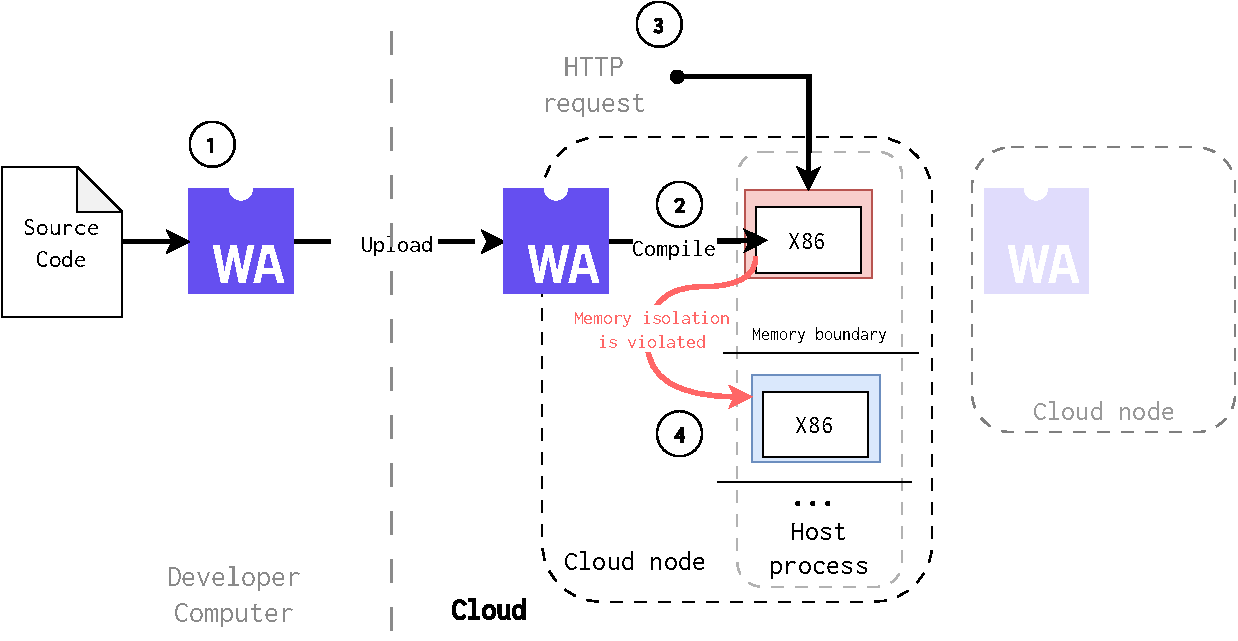
\includegraphics[width=0.8\linewidth]{figures/edge.pdf}
    \caption{\Wasm binaries on FaaS platforms.}
    \label{fig:edge_model}
\end{figure}


The fundamental advantage of using \Wasm in FaaS platforms lies in its ability to encapsulate thousands of client \Wasm binaries within a singular host process.
A developer could compile its source code into a \Wasm program suitable for the cloud platform and then submit it (\step{1} in \autoref{fig:edge_model}).
This host process is then disseminated across a network of servers and data centers (\step{2} in \autoref{fig:edge_model}). 
These platforms convert \Wasm programs into native code, which is subsequently executed in a sandboxed environment. 
Host processes can then instantiate new \Wasm sandboxes for each client function, executing them in response to specific user requests with nanosecond-level latency (\step{3} in \autoref{fig:edge_model}). 
This architecture inherently isolates \Wasm binary executions from each other as well as from the host process, enhancing security.

However, while \Wasm is engineered with a strong on security and isolation, it is not entirely immune to vulnerabilities such as Spectre attacks \cite{Spectre,Narayan2021Swivel} (\step{4} in \autoref{fig:edge_model}). 
In the sections that follow, we explore how software diversification techniques can be employed to fortify \Wasm binaries against such attacks. 
Specifically, we discuss the concept of Defensive Software Diversification, aimed at enhancing the security of \Wasm binaries by generating a multitude of diverse and unique \Wasm variants that can be randomized during deployment.
For an in-depth discussion on this topic, we direct the reader to our contribution \cite{wasmmutate}.

\msubsection{Threat model: speculative side-channel attacks}

To illustrate the threat model concerning \Wasm programs in FaaS platforms, consider the following scenarios. 
Developers, including potentially malicious actors, have the ability to submit any \Wasm binary to the FaaS platform. 
A malicious actor could upload a \Wasm binary that, once compiled to native code, employs Spectre attacks to either leak sensitive information from the host process or violate Control Flow Integrity (CFI).
Furthermore, even if a submitted \Wasm binary is not intentionally malicious, it may still be vulnerable to Spectre attacks. 
For instance, a malicious actor could exploit this vulnerability by executing the susceptible binary through the FaaS service. 

Spectre attacks exploit hardware-based prediction mechanisms to trigger mispredictions, leading to the speculative execution of specific instruction sequences that are not part of the original, sequential execution flow. 
By taking advantage of this speculative execution, an attacker can potentially access sensitive information stored in the memory allocated to other \Wasm instance(including itself) or even the host process itself. 
This poses a significant risk, compromising both the security and integrity of the overall system.

Narayan and colleagues \cite{Narayan2021Swivel} have categorized potential Spectre attacks on \wasm binaries into three distinct types, each corresponding to a specific hardware predictor being exploited and a particular FaaS scenario: Branch Target Buffer Attacks,  Return Stack Buffer Attacks, and Pattern History Table Attacks defined as follows:

\begin{enumerate}
    \item The Spectre Branch Target Buffer (btb) attack exploits the branch target buffer by predicting the target of an indirect jump, thereby rerouting speculative control flow to an arbitrary target.
    \item  The Spectre Return Stack Buffer (rsb) attack exploits the return stack buffer that stores the locations of recently executed call instructions to predict the target of \texttt{ret} instructions.
    \item The Spectre Pattern History Table (pht) takes advantage of the pattern history table to anticipate the direction of a conditional branch during the ongoing evaluation of a condition.
\end{enumerate}


%\lipsum[1]

%\lipsum[1]

\msubsection{Methodology}

Our goal is to empirically validate that Software Diversification can effectively mitigate the risks associated with Spectre attacks in \Wasm binaries. 
The green-highlighted section in \autoref{fig:defense_model} illustrates how Software Diversification can be integrated into the FaaS platform workflow. 
The core idea is to generate unique and diverse \Wasm variants that can be randomized at the time of deployment. 
For this use case, we employ WASM-MUTATE as our tool for Software Diversification.

To empirically demonstrate that Software Diversification can indeed mitigate Spectre vulnerabilities, we utilize the \Wasm binaries proposed by Narayan and colleagues in their work on Swivel \cite{Swivel}. 
Swivel is a compiler-based strategy designed to counteract Spectre attacks on \Wasm binaries by linearizing their control flow during machine code compilation. 
Our approach differs from theirs in that it is binary-based, compiler-agnostic, and platform-agnostic; we do not propose altering the deployment or toolchain of FaaS platforms. 
Although our experiments are conducted prior to submitting the \Wasm binary to the FaaS platform, we argue that \Wasm binary diversification could be implemented at any stage of the FaaS workflow.
The same argument holds by using any other diversification technique included in this dissertation (see \autoref{tech}).


\begin{figure}[h]
    \centering
    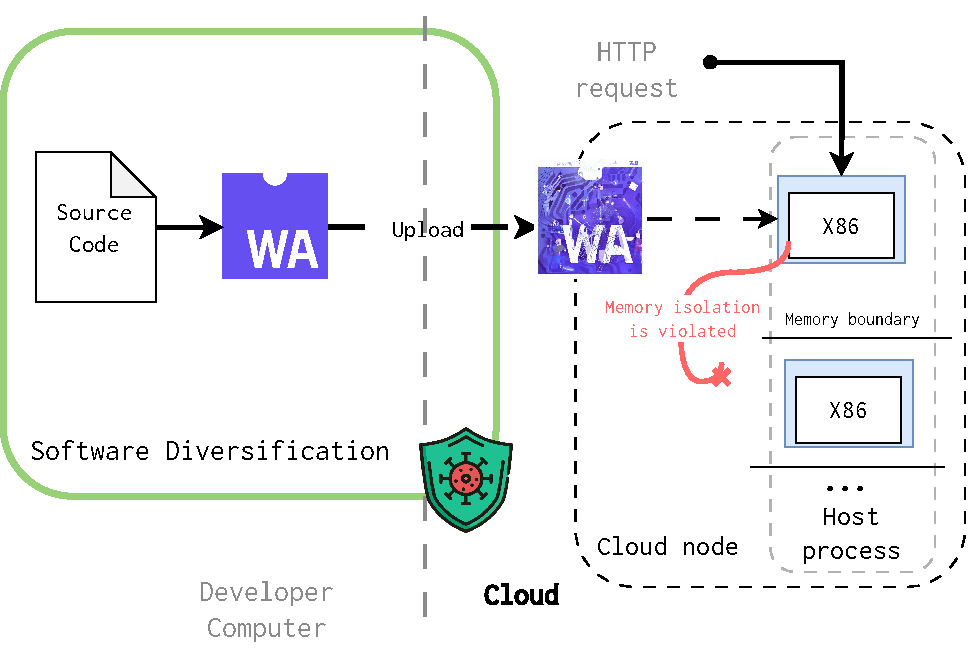
\includegraphics[width=0.75\linewidth]{figures/edge_protected.pdf}
    \caption{Diversifying \Wasm binaries to mitigate Spectre attacks in FaaS platforms.}
    \label{fig:defense_model}
\end{figure}

\begin{table}
    \centering
    \begin{tabular}{l | l  }
        \hline
         Program &  Attack  \\
        \hline \hline
        btb\_breakout & Spectre branch target buffer (btb)  \\
        \hline
         btb\_leakage & Spectre branch target buffer(btb)  \\
        \hline
         ret2spec &  Spectre Return Stack Buffer (rsb)  \\
        \hline
        pht &  Spectre Pattern History Table (pht)  \\

%\end{adjustbox}
    \end{tabular}
    \caption{}
    \label{programs}
\end{table}

To measure the efficacy of WASM-MUTATE in mitigating Spectre, we diversify four \Wasm binaries proposed in the Swivel study. 
The details of these programs and the specific attacks we examine are available in \cite{programs}. 
For each of these four binaries, we generate up to 1000 random stacked transformations using 100 distinct seeds, resulting in a total of 100,000 variants for each original binary. 
At every 100th stacked transformation for each binary and seed, we assess the impact of diversification on the Spectre attacks by measuring the attack bandwidth for data exfiltration. 
This metric not only captures the success or failure of the attacks but also quantifies the extent to which data exfiltration is hindered. 
For example, a variant that still leaks data but does so at an impractically slow rate would be considered hardened against the attack.

\begin{definition}{Attack bandwidth:}\label{metric:ber}
    Given data $D=\{b_0, b1, ..., b_C\}$ being exfiltrated in time $T$ and $K = {k_1, k_2, ..., k_N}$ the collection of correct data bytes, the bandwidth metric is defined as:
    $$
        \frac{|b_i\text{ such that } b_i \in K|}{T}
    $$
\end{definition}


\msubsection{Results}


\autoref{attacks:impact:1} offers a graphical representation of \tool's influence on the Swivel original programs: btb\_breakout and btb\_leakage with the btb attack. 
The Y-axis represents the exfiltration bandwidth (see \autoref{metric:ber}). 
The bandwidth of the original binary under attack is marked as a blue dashed horizontal line.
In each plot, the variants are grouped in clusters of 100 stacked transformations. 
These are indicated by green violinplots.

\begin{figure}[h]
    \centering
    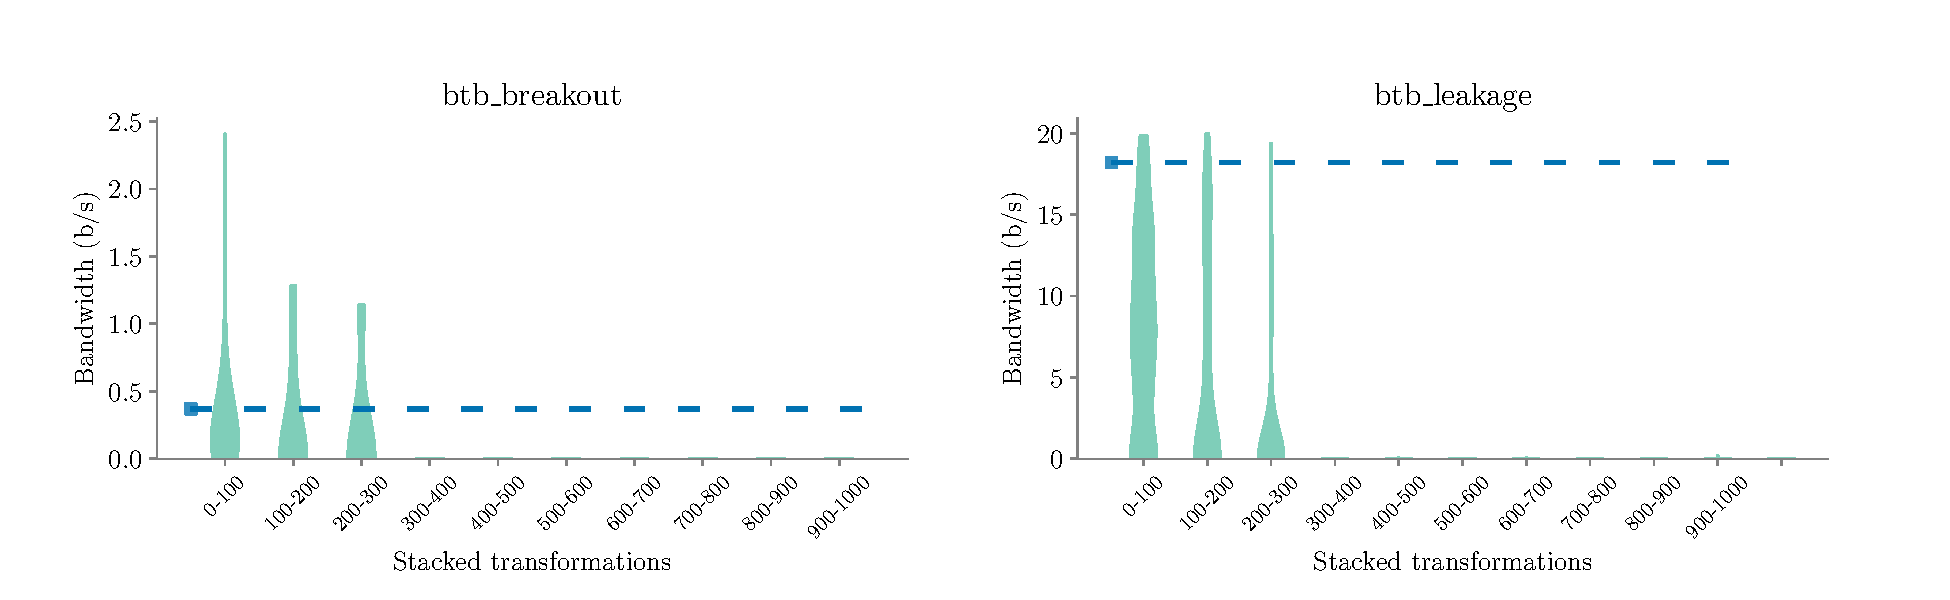
\includegraphics[width=\linewidth]{plots/spectre/results.rq3.1.pdf}
    \caption{TODO}
  \label{attacks:impact:1}
\end{figure}

\wrule{Population strength:} For btb\_breakout and btb\_leakage, \tool demonstrates effectiveness, generating variants that leak less information than the original in 78\% and 70\% of the cases, respectively.
For these particular binaries, a significant reduction in exfiltration bandwidth to zero is noted after 200 stacked transformations.
This means that with a minimum of 200 stacked transformations, \tool can create variants that are completely resistant to the original attack.
Comparing to \autoref{comp:table:tools}, a variant with 200 stacked transformations can be generated in merely minutes.



\begin{figure}[h]
    \centering    
    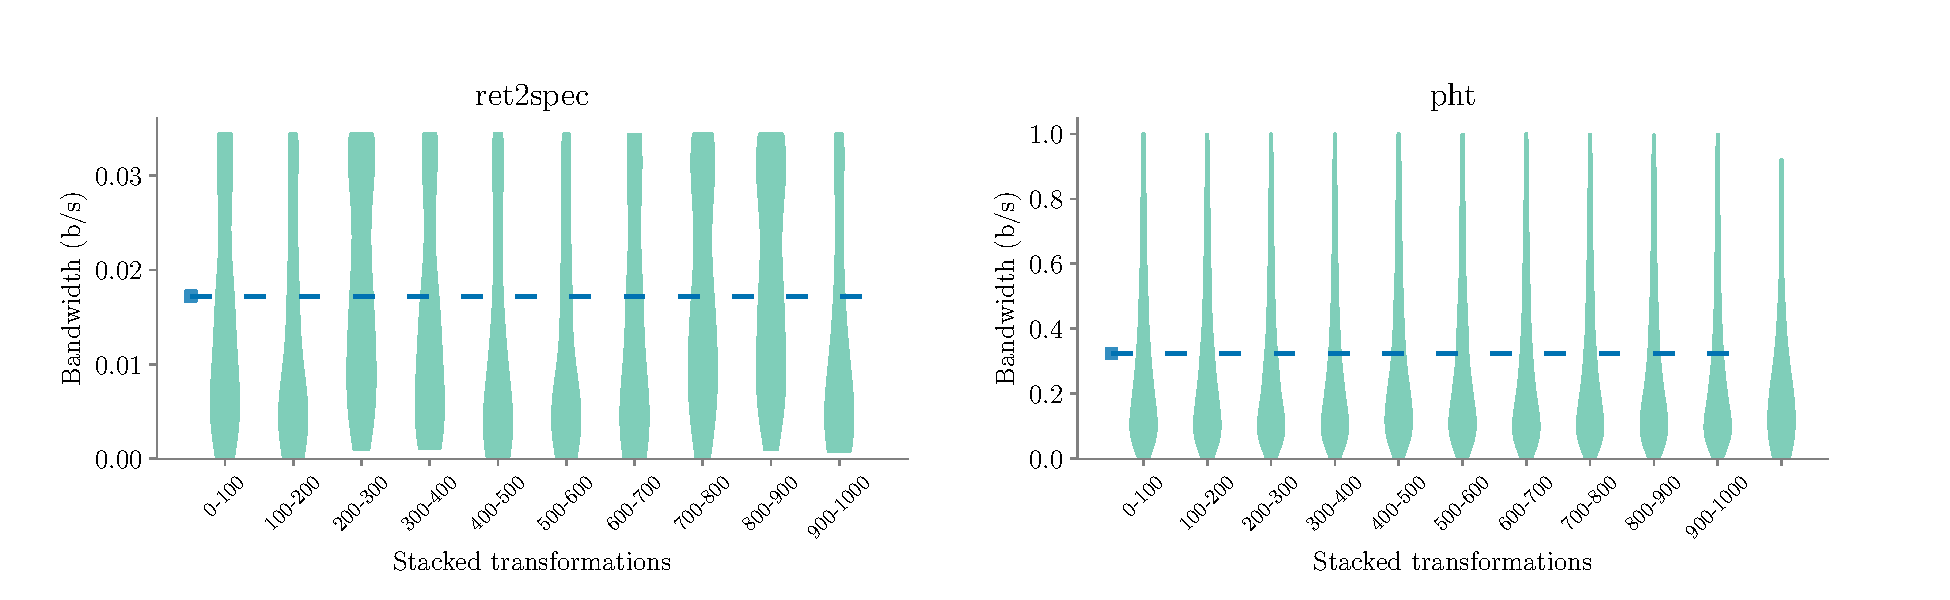
\includegraphics[width=\linewidth]{plots/spectre/results.rq3.2.pdf}
    \caption{TODO}
  \label{attacks:impact:2}
\end{figure}


% \todo{replace with violin plots}
\autoref{attacks:impact:2} offers a graphical representation of \tool's influence on the Swivel original programs: ret2spec and pht with the rest2spec and pht attacks respectively. 
For the ret2spec and pht scenarios, the produced variants consistently exhibit lower bandwidth than the original in 76\% and 71\% of instances, respectively.
% Why is good, for breaking timers and for padding
As depicted in the plots, the exfiltration bandwidth diminishes following the application of at least  100 stacked transformations.
Both programs are hardened with attack bandwidth reduction, but this does not materialize in a short-term timeframe (low count of stacked transformations).
Furthermore,  the exfiltration bandwidth is more dispersed for these two programs.
Our analysis indicates a correlation between bandwidth reduction and the complexity of the binary subject to diversification.
Ret2spec and pht are considerably larger than btb\_breakout and btb\_leakage.
The former comprises more than 300k instructions, while the latter two include fewer than 800 instructions.
Given that WASM-MUTATE applies precise, fine-grained transformations one at a time, the likelihood of impacting critical attack components, such as timing memory accesses, diminishes for larger binaries, particularly when limited to 1000 transformations.
Based on these observations, we believe that a greater number of stacked transformations would further contribute to eventually eliminating the attacks associated with ret2spec and pht.

\wrule{Managed memory impact:} The success in diminishing exfiltration is explained by the fact that \tool synthesizes variants that effectively alter memory access patterns. 
Specifically, it does so by amplifying spill/reload operations, injecting artificial global variables, and changing the frequency of pre-existing memory accesses. 
These transformations influence the \wasm program's memory (as discussed in \autoref{security_applications}), causing disruption to cache predictors. 
As a result, these alterations contribute to a reduction in exfiltration bandwidth.

% More fine grained
\wrule{Disrupting accurate timers:} Furthermore, many attacks rely on a timer component to measure cache access time for memory, and disrupting this component  effectively impairs the attack's effectiveness. 
This strategy of dynamic alteration has also been  employed in other scenarios. 
For instance, to counter potential timing attacks, Firefox randomizes its built-in JavaScript timer \cite{10.1007/978-3-319-70972-7_13}. \tool applies the same strategy by interspersing instructions within the timing steps of \wasm variants. 
In \autoref{example:timer} and \autoref{example:timer2}, we demonstrate \tool's impact on time measurements. 
The former illustrates the original time measurement, while the latter presents a variant with \tool-inserted operations amid the timing.


\lstdefinestyle{watcode}{
  numbers=none,
  stepnumber=1,
  numbersep=10pt,
  tabsize=4,
  showspaces=false,
  breaklines=true, 
  showstringspaces=false,
    moredelim=**[is][{\btHL[fill=weborange!40]}]{`}{`},
    moredelim=**[is][{\btHL[fill=celadon!40]}]{!}{!}
}


   \begin{minipage}[b]{\linewidth}
    \lstset{
        language=WAT,
                        style=watcode,
        basicstyle=\footnotesize\ttfamily,
                        columns=fullflexible,
                        breaklines=true}
        
        \begin{lstlisting}[label=example:timer,caption={Wasm timer code.},frame=b, captionpos=b]{Name}
;; Code from original btb_breakout
...
(call $readTimer)
(set_local $end_time)
... access to mem
(i64.sub (get_local $end_time ) (get_local $start_time))
(set_local $duration)
...

        \end{lstlisting}
\end{minipage}


\begin{minipage}[b]{\linewidth}
    \lstset{
        language=WAT,
                        style=watcode,
        basicstyle=\footnotesize\ttfamily,
                        columns=fullflexible,
                        breaklines=true}
        
        \begin{lstlisting}[label=example:timer2,caption={\Wasm variant with more instructions added in between time measurement.},frame=b, captionpos=b]{Name}
;; Variant code
...
(call $readTimer)
(set_local $end_time)
!<inserted instructions>!
... access to mem
!<inserted instructions>!
(i64.sub (get_local $end_time ) (get_local $start_time))
(set_local $duration)
...
        \end{lstlisting}
\end{minipage}


WASM-MUTATE proves effective against cache access timers because the time measurement of single or a few instructions is inherently different. 
By introducing more instructions, this randomness is amplified, thereby reducing the timer's accuracy.
Furthermore, CPUs have a maximum capacity for the number of instructions they can cache.
\tool injects instructions in such a way that the vulnerable instruction may exceed this cacheable instruction limit, meaning that caching becomes disabled.
This kind of transformation can be viewed as padding \cite{padding}.
In \autoref{example:padding} and \autoref{example:padding2}, we illustrate the effect of \tool on padding instructions.
\autoref{example:padding} presents the original code used for training the branch predictor, along with the expected speculated code.


\lstdefinestyle{watcode}{
  numbers=none,
  stepnumber=1,
  numbersep=10pt,
  tabsize=4,
  showspaces=false,
  breaklines=true, 
  showstringspaces=false,
    moredelim=**[is][{\btHL[fill=weborange!40]}]{`}{`},
    moredelim=**[is][{\btHL[fill=celadon!40]}]{!}{!}
}


   \begin{minipage}[b]{0.8\linewidth}
    \lstset{
        language=WAT,
                        style=watcode,
        basicstyle=\footnotesize\ttfamily,
                        columns=fullflexible,
                        breaklines=true}
        
        \begin{lstlisting}[label=example:padding,caption={Two jump locations. The top one trains the branch predictor, the bottom one is the expected jump that exfiltrates the memory access.},frame=b, captionpos=b]{Name}
;; Code from original btb_breakout
...
;; train the code to jump here (index 1)
(i32.load (i32.const 2000))
(i32.store (i32.const 83)) ;; just prevent optimization
...
;; transiently jump here
(i32.load (i32.const 339968)) ;; S(83) is the secret
(i32.store (i32.const 83)) ;; just prevent optimization
        \end{lstlisting}
\end{minipage}


\begin{minipage}[b]{0.8\linewidth}
    \lstset{
        language=WAT,
                        style=watcode,
        basicstyle=\footnotesize\ttfamily,
                        columns=fullflexible,
                        breaklines=true}
        
        \begin{lstlisting}[label=example:padding2,caption={\Wasm variant with more instructions added indindinctly between jump places.},frame=b, captionpos=b]{Name}
;; Variant code
...
;; train the code to jump here (index 1)
!<inserted instructions>!
(i32.load (i32.const 2000))
!<inserted instructions>!
(i32.store (i32.const 83)) ;; just prevent optimization
...
;; transiently jump here
!<inserted instructions>!
(i32.load (i32.const 339968)) ;; "S"(83) is the secret
!<inserted instructions>!
(i32.store (i32.const 83)) ;; just prevent optimization
...
        \end{lstlisting}
\end{minipage}


The padding alters the arrangement of the binary code in memory, effectively impeding the attacker's capacity to initiate speculative execution.
Even when an attack is launched and the vulnerable code is "speculated", the memory access is not impacted as planned.


In every program, we note that the exfiltration bandwidth tends to be greater than the original when the variants include a few transformations.
This indicates that, although the transformations generally contribute to the reduction of data leakage, the initial few might not consistently contribute positively towards this objective.
We have identified several fundamental reasons, which we discuss below.

Firstly, as emphasized previously in \autoref{offensive_app}, uncontrolled diversification can be counterproductive if a specific objective, such as a cost function, is not established at the beginning of the diversification process.
Secondly, while some transformations yield distinct \wasm binaries, their compilation produces identical machine code.
Transformations that are not preserved(see \autoref{discussion}) undermine the effectiveness of diversification.
For example, incorporating random \texttt{nop} operations directly into \wasm does not modify the final machine code as the \texttt{nop} operations are often removed by the compiler.
The same phenomenon is observed with transformations to custom sections of \Wasm binaries.
Additionally, it is important to note that transformed code doesn't always execute, i.e., \tool may generate dead code.





% \subsection{Deoptimization}

\begin{tcolorbox}[title=Contribution paper,boxrule=1pt,arc=.2em,boxsep=1.0mm]
    Software diversification is effective at synthesizing \wasm binaries that mitigate Spectre-like attacks. 
    The case discussed in this section is fully detailed in Cabrera-Arteaga \etal "WASM-MUTATE: Fast and Effective Binary Diversification for WebAssembly"
    \emph{Under review}
    \url{https://arxiv.org/pdf/2309.07638.pdf}. 
\end{tcolorbox}



